\documentclass[12pt]{article}

\usepackage{hyperref}
\usepackage{graphicx}
\usepackage{titling}

\setlength{\droptitle}{-10em}

\title
{ 
    G53IDS - Project Proposal \\
    \hfill \break
    \large Embedded Domain Specific Language for \\
    Describing Recipes in Haskell
}

\author{James Burton - 4251529 - psyjb6}

\begin{document}
    \maketitle

    \section{Background and Motivation}

    The need for food is one of the few things that everyone has in
    common. Recipes are therefore a domain of great relevance. Being able
    to model a domain on a computer is incredibly useful as we are then
    able to do anything from computer aided decision making to straight
    up automation. \\

    
    Domain Specific Languages (DSLs) are an incredibly powerful way of
    modeling a problem domain. "A well-designed DSL captures precisely
    the semantics of an application domain, no more and no less." \cite{hudak}.
    This means that not only is the representation of the problem domain
    more concise, as it cuts out the "noise" of a general purpose language,
    but it also opens up the potential for non-programmers to use the
    language. One of the most popular DSLs is HTML for describing
    web pages. \\
    
    
    The type of DSL that is relevant to this project is an Embedded
    Domain Specific Language (EDSL) where the DSL is defined inside
    another programming language. \cite{hudak} expresses several advantages to
    this among which is "rapid DSL design" as there is no need to
    build a parser for the language. \\


    For this project, Haskell shall be the language in which the EDSL is
    embedded. Haskell has become a popular choice for EDSLs being used
    to create DSLs for financial contracts \cite{contracts} and pretty
    printing \cite{pretty} to name a few. Michael Snoyman, creator of
    Yesod (a Haskell Web Framework), stated many advantages of using
    Haskell for EDSLs among which were that the type system helps catch
    mistakes and Haskell allows us to overload almost any syntax
    \cite{snoyman}. \\

    A DSL describing recipes would thus be very useful. A few uses that
    come to mind are:

    \begin{itemize}

        \item The creation of a shopping list from a set of
        recipes, this would save people time and potentially prevent them
        forgetting things.

        \item Programming machines that produce food.

        \item Creating the backend of a website about food, perhaps
        integrating the shopping list generator.

        \item Academic research into recipes and the combinations
        of ingredients that do and don't work and other "cheffy"
        things.

    \end{itemize}

    It is thus surprising that no such DSL exists, or at least none
    that I could find. Perhaps this is testament to how much food,
    as important as it is, oft becomes an after thought in todays
    hectic society.

    \section{Aims and Objectives}

    The aim of this project is to create an EDSL in Haskell to describe
    recipes. The main objectives are:

    \begin{enumerate}

        \item Research DSLs, particularly EDSLs in Haskell to gain
        an understanding of the design process hopefully allowing
        the avoidance of common mistakes.

        \item Consider a small selection of recipes and extract
        common features.

        \item Map these common features to a set of combinators
        and attempt to build a wider more complex set of recipes,
        adjusting the combinators if necessary.

        \item Consider the potential representations of a recipe,
        e.g. functionaly or as a data type.

        \item Investigate the algebraic properties of the
        combinators and ensure the DSL supports these. Potentially
        write the properties using QuickCheck.

        \item Consider and create other non-core features of the DSL
        such as:

            \begin{itemize}

                \item Printing of recipes in the DSL to a format that
                you would see in a recipe book.

                \item Parser to read recipe formatted input
                into the DSL.

                \item Tools to manipulate recipes such as determining
                which steps could be executed in parallel or generating
                a shopping list as described earlier.

            \end{itemize}

    \end{enumerate}

    \section{Project Plan}

    This project shall use the scrum development methodology. With the
    gaps between supervisor meetings acting as the sprints. The scrum
    methodology seems most appropriate for this project as it is naturally
    very flexibly and doesn't require a huge amount of detailed planning
    in advance. This suits the research nature of the project as it is
    impossible to precisely state what will be done and when. Each sprint
    offers an opporuntity to re-prioritise and alter tasks based upon
    the progress and findings of the previous sprint.

    \begin{enumerate}

        \item Create project proposal and email to supervisor
        (deadline 13th October).

        \item Submit completed ethics clearance form to supervisor
        (deadline 23rd October).

        \item Amend project proposal based on feedback from
        supervisor and submit amended version (deadline 23rd October).

        \item Read \cite{hudak, contracts, pretty} to gain a better
        understanding of the DSL design process.

        \item Boil down, if you'll forgive the pun, a few recipes
        into their components and recreate the recipes in terms
        of a set of combinators. Try to create other more complex
        recipes and repeat until a satisfactory set of combinators
        is found.

        \item Define algebraic properties of the combinators.

        \item Consider various representations of recipes and the
        combinators e.g. as functions or as data structures.

        \item Write and submit interim report (deadline 8th December).

        \item Mainly revise for other modules over Christmas and during
        exams.

        \item Once the core components of the DSL are in place
        consider specifics such as temperature being centigrade,
        farenheit or gas mark.

        \item Create system to output recipes from the DSL into a format
        similar to that of a regular recipe.

        \item Create parser to read recipe formatted text into the DSL.

        \item Experiment with various applications of the DSL such
        as finding steps that can be executed concurrently.

        \item Outline contents for final report.

        \item Write and submit final report (deadline 24th April).

    \end{enumerate}

    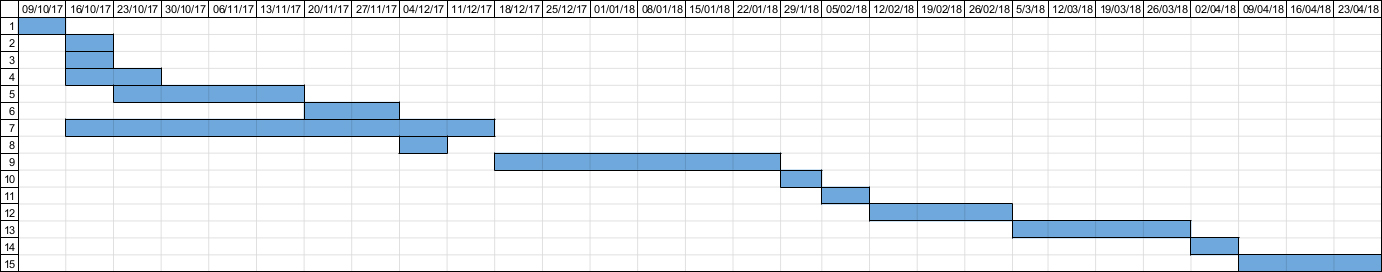
\includegraphics[width=\textwidth,keepaspectratio]{gantt_chart.jpg}
    
    \begin{thebibliography}{4}
    
        \bibitem{hudak}
        Paul Hudak. Domain Specific Languages. Department of Computer
        Science, Yale University, December 15, 1997.

        \bibitem{contracts}
        Simon Peyton Jones, Microsoft Research, Cambridge.
        Jean-Marc Eber, LexiFi Technologies, Paris. Julian Seward,
        University of Glasgow. Composing contracts: an adventure in
        financial engineering. August 17, 2000.

        \bibitem{pretty}
        John Hughes. The Design of a Pretty-printing Library.
        Chalmers Teniska Hogskola, Goteborg, Sweden. 1995.

        \bibitem{snoyman}
        Michael Snoynman. O'Reilly Webcast: Designing Domain Specific
        Languages with Haskell. January 4, 2013.
        \url{https://www.youtube.com/watch?v=8k_SU1t50M8}

    \end{thebibliography}

\end{document}